% python classes slides - profiling and optimization
% (c) 2014 Kostiantyn Danylov aka koder 
% koder.mail@gmail.com
% distributed under CC-BY licence
% http://creativecommons.org/licenses/by/3.0/deed.en

\documentclass{article}
% XeLaTeX
\usepackage{xltxtra}
\usepackage{xunicode}
\usepackage{listings}
\usepackage[landscape]{geometry}

% Fonts
\setmainfont{DejaVu Sans} %{Arial}
\newfontfamily\cyrillicfont{Nimbus Roman No9 L} %{Arial}
\setmonofont{Courier New}
%\setmonofont{Ubuntu Mono}

%\setmonofont{DejaVu Sans Mono}

% Lang
\usepackage{polyglossia}
\setmainlanguage{russian}
\setotherlanguage{english}
\usepackage[dvipsnames,table]{xcolor}


\ifx\pdfoutput\undefined
\usepackage{graphicx}
\else
\usepackage[pdftex]{graphicx}
\fi

\lstset{
	language=python,
	keywordstyle=\color{Emerald},%\texttt, 
	commentstyle=\color{OliveGreen},%\texttt,
	stringstyle=\color{Bittersweet},%\texttt,
	tabsize=4,
	numbers=left,
	xleftmargin=10pt,
	morekeywords={with,as},	
	numberstyle=\large,
	%identifierstyle=\texttt,
	%basicstyle=\texttt,
}

\usepackage{hyperref}

\hypersetup{
	colorlinks=true,
	urlcolor=blue
}

\usepackage{float}
%\floatstyle{boxed} 
%\restylefloat{figure}
\usepackage[normalem]{ulem}


\makeatletter
\def\PY@reset{\let\PY@it=\relax \let\PY@bf=\relax%
    \let\PY@ul=\relax \let\PY@tc=\relax%
    \let\PY@bc=\relax \let\PY@ff=\relax}
\def\PY@tok#1{\csname PY@tok@#1\endcsname}
\def\PY@toks#1+{\ifx\relax#1\empty\else%
    \PY@tok{#1}\expandafter\PY@toks\fi}
\def\PY@do#1{\PY@bc{\PY@tc{\PY@ul{%
    \PY@it{\PY@bf{\PY@ff{#1}}}}}}}
\def\PY#1#2{\PY@reset\PY@toks#1+\relax+\PY@do{#2}}

\expandafter\def\csname PY@tok@gd\endcsname{\def\PY@tc##1{\textcolor[rgb]{0.63,0.00,0.00}{##1}}}
\expandafter\def\csname PY@tok@gu\endcsname{\let\PY@bf=\textbf\def\PY@tc##1{\textcolor[rgb]{0.50,0.00,0.50}{##1}}}
\expandafter\def\csname PY@tok@gt\endcsname{\def\PY@tc##1{\textcolor[rgb]{0.00,0.25,0.82}{##1}}}
\expandafter\def\csname PY@tok@gs\endcsname{\let\PY@bf=\textbf}
\expandafter\def\csname PY@tok@gr\endcsname{\def\PY@tc##1{\textcolor[rgb]{1.00,0.00,0.00}{##1}}}
\expandafter\def\csname PY@tok@cm\endcsname{\let\PY@it=\textit\def\PY@tc##1{\textcolor[rgb]{0.25,0.50,0.50}{##1}}}
\expandafter\def\csname PY@tok@vg\endcsname{\def\PY@tc##1{\textcolor[rgb]{0.10,0.09,0.49}{##1}}}
\expandafter\def\csname PY@tok@m\endcsname{\def\PY@tc##1{\textcolor[rgb]{0.40,0.40,0.40}{##1}}}
\expandafter\def\csname PY@tok@mh\endcsname{\def\PY@tc##1{\textcolor[rgb]{0.40,0.40,0.40}{##1}}}
\expandafter\def\csname PY@tok@go\endcsname{\def\PY@tc##1{\textcolor[rgb]{0.50,0.50,0.50}{##1}}}
\expandafter\def\csname PY@tok@ge\endcsname{\let\PY@it=\textit}
\expandafter\def\csname PY@tok@vc\endcsname{\def\PY@tc##1{\textcolor[rgb]{0.10,0.09,0.49}{##1}}}
\expandafter\def\csname PY@tok@il\endcsname{\def\PY@tc##1{\textcolor[rgb]{0.40,0.40,0.40}{##1}}}
\expandafter\def\csname PY@tok@cs\endcsname{\let\PY@it=\textit\def\PY@tc##1{\textcolor[rgb]{0.25,0.50,0.50}{##1}}}
\expandafter\def\csname PY@tok@cp\endcsname{\def\PY@tc##1{\textcolor[rgb]{0.74,0.48,0.00}{##1}}}
\expandafter\def\csname PY@tok@gi\endcsname{\def\PY@tc##1{\textcolor[rgb]{0.00,0.63,0.00}{##1}}}
\expandafter\def\csname PY@tok@gh\endcsname{\let\PY@bf=\textbf\def\PY@tc##1{\textcolor[rgb]{0.00,0.00,0.50}{##1}}}
\expandafter\def\csname PY@tok@ni\endcsname{\let\PY@bf=\textbf\def\PY@tc##1{\textcolor[rgb]{0.60,0.60,0.60}{##1}}}
\expandafter\def\csname PY@tok@nl\endcsname{\def\PY@tc##1{\textcolor[rgb]{0.63,0.63,0.00}{##1}}}
\expandafter\def\csname PY@tok@nn\endcsname{\let\PY@bf=\textbf\def\PY@tc##1{\textcolor[rgb]{0.00,0.00,1.00}{##1}}}
\expandafter\def\csname PY@tok@no\endcsname{\def\PY@tc##1{\textcolor[rgb]{0.53,0.00,0.00}{##1}}}
\expandafter\def\csname PY@tok@na\endcsname{\def\PY@tc##1{\textcolor[rgb]{0.49,0.56,0.16}{##1}}}
\expandafter\def\csname PY@tok@nb\endcsname{\def\PY@tc##1{\textcolor[rgb]{0.00,0.50,0.00}{##1}}}
\expandafter\def\csname PY@tok@nc\endcsname{\let\PY@bf=\textbf\def\PY@tc##1{\textcolor[rgb]{0.00,0.00,1.00}{##1}}}
\expandafter\def\csname PY@tok@nd\endcsname{\def\PY@tc##1{\textcolor[rgb]{0.67,0.13,1.00}{##1}}}
\expandafter\def\csname PY@tok@ne\endcsname{\let\PY@bf=\textbf\def\PY@tc##1{\textcolor[rgb]{0.82,0.25,0.23}{##1}}}
\expandafter\def\csname PY@tok@nf\endcsname{\def\PY@tc##1{\textcolor[rgb]{0.00,0.00,1.00}{##1}}}
\expandafter\def\csname PY@tok@si\endcsname{\let\PY@bf=\textbf\def\PY@tc##1{\textcolor[rgb]{0.73,0.40,0.53}{##1}}}
\expandafter\def\csname PY@tok@s2\endcsname{\def\PY@tc##1{\textcolor[rgb]{0.73,0.13,0.13}{##1}}}
\expandafter\def\csname PY@tok@vi\endcsname{\def\PY@tc##1{\textcolor[rgb]{0.10,0.09,0.49}{##1}}}
\expandafter\def\csname PY@tok@nt\endcsname{\let\PY@bf=\textbf\def\PY@tc##1{\textcolor[rgb]{0.00,0.50,0.00}{##1}}}
\expandafter\def\csname PY@tok@nv\endcsname{\def\PY@tc##1{\textcolor[rgb]{0.10,0.09,0.49}{##1}}}
\expandafter\def\csname PY@tok@s1\endcsname{\def\PY@tc##1{\textcolor[rgb]{0.73,0.13,0.13}{##1}}}
\expandafter\def\csname PY@tok@sh\endcsname{\def\PY@tc##1{\textcolor[rgb]{0.73,0.13,0.13}{##1}}}
\expandafter\def\csname PY@tok@sc\endcsname{\def\PY@tc##1{\textcolor[rgb]{0.73,0.13,0.13}{##1}}}
\expandafter\def\csname PY@tok@sx\endcsname{\def\PY@tc##1{\textcolor[rgb]{0.00,0.50,0.00}{##1}}}
\expandafter\def\csname PY@tok@bp\endcsname{\def\PY@tc##1{\textcolor[rgb]{0.00,0.50,0.00}{##1}}}
\expandafter\def\csname PY@tok@c1\endcsname{\let\PY@it=\textit\def\PY@tc##1{\textcolor[rgb]{0.25,0.50,0.50}{##1}}}
\expandafter\def\csname PY@tok@kc\endcsname{\let\PY@bf=\textbf\def\PY@tc##1{\textcolor[rgb]{0.00,0.50,0.00}{##1}}}
\expandafter\def\csname PY@tok@c\endcsname{\let\PY@it=\textit\def\PY@tc##1{\textcolor[rgb]{0.25,0.50,0.50}{##1}}}
\expandafter\def\csname PY@tok@mf\endcsname{\def\PY@tc##1{\textcolor[rgb]{0.40,0.40,0.40}{##1}}}
\expandafter\def\csname PY@tok@err\endcsname{\def\PY@bc##1{\setlength{\fboxsep}{0pt}\fcolorbox[rgb]{1.00,0.00,0.00}{1,1,1}{\strut ##1}}}
\expandafter\def\csname PY@tok@kd\endcsname{\let\PY@bf=\textbf\def\PY@tc##1{\textcolor[rgb]{0.00,0.50,0.00}{##1}}}
\expandafter\def\csname PY@tok@ss\endcsname{\def\PY@tc##1{\textcolor[rgb]{0.10,0.09,0.49}{##1}}}
\expandafter\def\csname PY@tok@sr\endcsname{\def\PY@tc##1{\textcolor[rgb]{0.73,0.40,0.53}{##1}}}
\expandafter\def\csname PY@tok@mo\endcsname{\def\PY@tc##1{\textcolor[rgb]{0.40,0.40,0.40}{##1}}}
\expandafter\def\csname PY@tok@kn\endcsname{\let\PY@bf=\textbf\def\PY@tc##1{\textcolor[rgb]{0.00,0.50,0.00}{##1}}}
\expandafter\def\csname PY@tok@mi\endcsname{\def\PY@tc##1{\textcolor[rgb]{0.40,0.40,0.40}{##1}}}
\expandafter\def\csname PY@tok@gp\endcsname{\let\PY@bf=\textbf\def\PY@tc##1{\textcolor[rgb]{0.00,0.00,0.50}{##1}}}
\expandafter\def\csname PY@tok@o\endcsname{\def\PY@tc##1{\textcolor[rgb]{0.40,0.40,0.40}{##1}}}
\expandafter\def\csname PY@tok@kr\endcsname{\let\PY@bf=\textbf\def\PY@tc##1{\textcolor[rgb]{0.00,0.50,0.00}{##1}}}
\expandafter\def\csname PY@tok@s\endcsname{\def\PY@tc##1{\textcolor[rgb]{0.73,0.13,0.13}{##1}}}
\expandafter\def\csname PY@tok@kp\endcsname{\def\PY@tc##1{\textcolor[rgb]{0.00,0.50,0.00}{##1}}}
\expandafter\def\csname PY@tok@w\endcsname{\def\PY@tc##1{\textcolor[rgb]{0.73,0.73,0.73}{##1}}}
\expandafter\def\csname PY@tok@kt\endcsname{\def\PY@tc##1{\textcolor[rgb]{0.69,0.00,0.25}{##1}}}
\expandafter\def\csname PY@tok@ow\endcsname{\let\PY@bf=\textbf\def\PY@tc##1{\textcolor[rgb]{0.67,0.13,1.00}{##1}}}
\expandafter\def\csname PY@tok@sb\endcsname{\def\PY@tc##1{\textcolor[rgb]{0.73,0.13,0.13}{##1}}}
\expandafter\def\csname PY@tok@k\endcsname{\let\PY@bf=\textbf\def\PY@tc##1{\textcolor[rgb]{0.00,0.50,0.00}{##1}}}
\expandafter\def\csname PY@tok@se\endcsname{\let\PY@bf=\textbf\def\PY@tc##1{\textcolor[rgb]{0.73,0.40,0.13}{##1}}}
\expandafter\def\csname PY@tok@sd\endcsname{\let\PY@it=\textit\def\PY@tc##1{\textcolor[rgb]{0.73,0.13,0.13}{##1}}}

\def\PYZbs{\char`\\}
\def\PYZus{\char`\_}
\def\PYZob{\char`\{}
\def\PYZcb{\char`\}}
\def\PYZca{\char`\^}
\def\PYZam{\char`\&}
\def\PYZlt{\char`\<}
\def\PYZgt{\char`\>}
\def\PYZsh{\char`\#}
\def\PYZpc{\char`\%}
\def\PYZdl{\char`\$}
\def\PYZti{\char`\~}
% for compatibility with earlier versions
\def\PYZat{@}
\def\PYZlb{[}
\def\PYZrb{]}
\makeatother

\begin{document}
\LARGE

%-------------------------------------------------------------------------------
\begin{center} TCP level networking \end{center}
\newpage

%-------------------------------------------------------------------------------
\begin{center} Стек протоколов \end{center}
\begin{itemize}
    \item Ethernet
    \item IP
    \item TCP/UDP
    \item HTTP/FTP/SSH/...
\end{itemize}
\newpage

%-------------------------------------------------------------------------------
\begin{center} ISO vs. ANSI \end{center}
\newpage

%-------------------------------------------------------------------------------
\begin{center} IP \end{center}
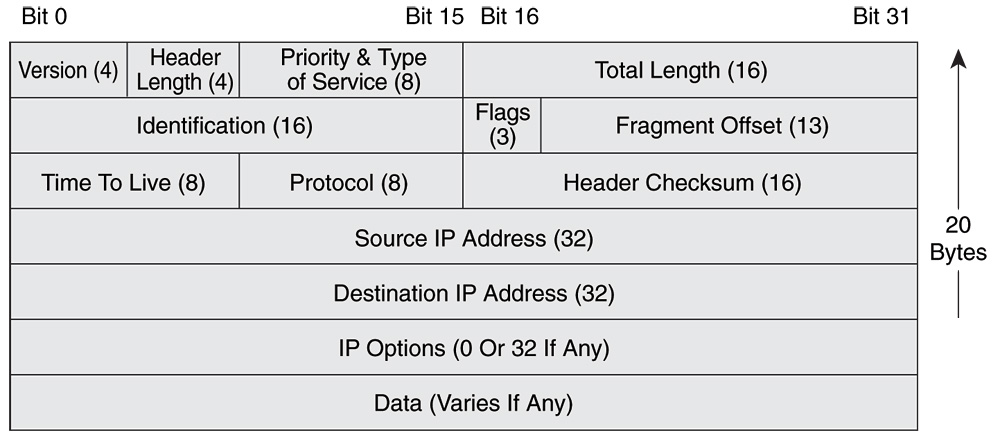
\includegraphics[scale=0.6]{images/ip_header.jpg}
\newpage

%-------------------------------------------------------------------------------
\begin{center} TCP/UDP \end{center}
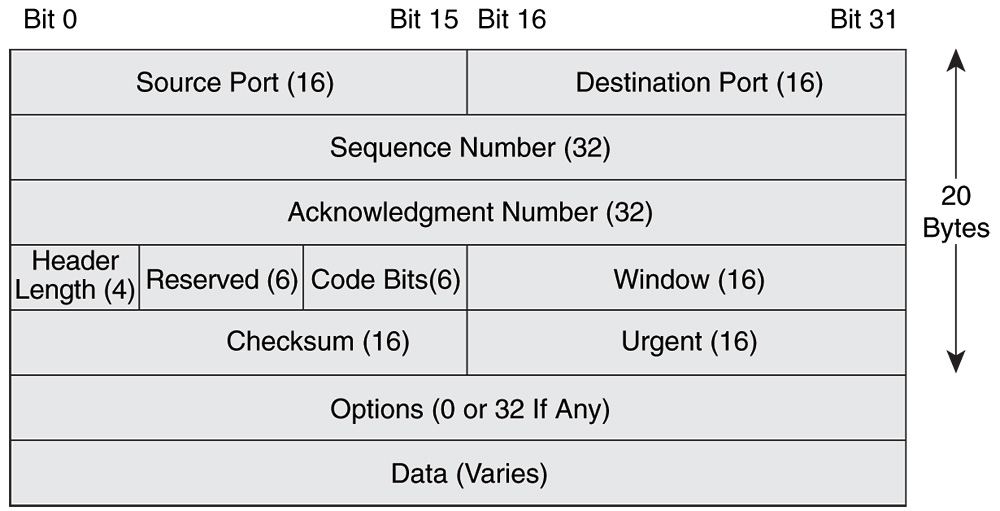
\includegraphics[scale=0.6]{images/tcpheader.jpg}
\newpage

%-------------------------------------------------------------------------------
\begin{center} Python TCP client \end{center}
\begin{lstlisting}
import socket

with socket.socket(socket.AF_INET, socket.SOCK_STREAM) as s:  # tcp by default
    s.connect(('127.0.0.1', 12345))  # ip or hostname
    s.send("Hello, World!".encode('utf8'))

    # 1
    print("Recv", s.recv(1024).decode('utf8'))

    # 2
    # fd = s.makefile()
    # fd.read()
\end{lstlisting}
\newpage


%-------------------------------------------------------------------------------
\begin{center} Python TCP server \end{center}
\begin{lstlisting}
import socket

sz = 32

with socket.socket() as s:
    s.bind(('', 12345))
    s.listen(1)

    conn, addr = s.accept()
    print('Connection address:', addr)
    while True:
        data = conn.recv(sz)
        if not data:
            break
        print("received data:", data.decode('utf8'))
        conn.send(data)
\end{lstlisting}
\newpage

%-------------------------------------------------------------------------------
\begin{center} БД/DB2 API \end{center}
\begin{itemize}
    \item Connection (commit/rollback)
    \item Cursor (execute/fetchone/fetchall/executemany)
    \item Транзакция
\end{itemize}
\newpage

%-------------------------------------------------------------------------------
\begin{center} sqlite3 \end{center}
\begin{lstlisting}
import sqlite3

conn = sqlite3.connect('/tmp/data.db')
cursor = conn.cursor()
conn.close()

\end{lstlisting}
\newpage

%-------------------------------------------------------------------------------
\begin{center} sqlite3 \end{center}
\begin{lstlisting}
import sqlite3

def prepare(cr):
    try:
        cr.execute("select key from messages limit 1")
    except sqlite3.OperationalError:
        cr.execute("create table messages (key text primary key, msg text)")


def show_db(cr):
    cr.execute("select key, msg from messages")
    print("\n#-----------------------")
    for key, msg in cr.fetchall():
        print(">>>", key, msg)
    print("#-----------------------\n")
\end{lstlisting}
\newpage

%-------------------------------------------------------------------------------
\begin{center} sqlite3 \end{center}
\begin{lstlisting}
conn = sqlite3.connect("/tmp/data.db")
cr = conn.cursor()
show_db(cr)
prepare(cr)
conn.commit()

cr = conn.cursor()
cr.execute("insert into messages values (?, ?)", ("1", "this will disappears"))
show_db(cr)
conn.rollback()
show_db(conn.cursor())


cr = conn.cursor()
cr.execute("insert into messages values (?, ?)", ("2", "this will remains"))
show_db(cr)
conn.commit()
show_db(conn.cursor())
\end{lstlisting}
\newpage

%-------------------------------------------------------------------------------
\begin{center} sqlite3 \end{center}
\begin{lstlisting}
import contextlib

@contextlib.contextmanager
def transaction(conn):
    cr = conn.cursor()
    try:
        yield cr
    except:
        conn.rollback()
        raise
    conn.commit()
\end{lstlisting}
\newpage


%-------------------------------------------------------------------------------
\begin{center} sqlite3 \end{center}
\begin{lstlisting}
with transaction(conn) as cr:
    cr.execute("insert into messages values (?, ?)", ("5", "this will also remains"))

with transaction(conn) as cr:
    show_db(cr)

with transaction(conn) as cr:
    cr.execute("insert into messages values (?, ?)", ("6", "this will not remains"))
    show_db(cr)
    raise ValueError("")

with transaction(conn) as cr:
    show_db(cr)
\end{lstlisting}
\newpage

%-------------------------------------------------------------------------------
\begin{center} sqlite3 \end{center}
\begin{lstlisting}
data = [(str(x), "msg {}".format(x)) for x in range(10, 20)]
with transaction(conn) as cr:
    cr.executemany("insert into messages values (?, ?)", data)
\end{lstlisting}
\newpage

%-------------------------------------------------------------------------------
\begin{center} sqlite3 \end{center}
\begin{lstlisting}
from sqlalchemy import Column, String
from sqlalchemy.ext.declarative import declarative_base

Base = declarative_base()

class Message(Base):
    __tablename__ = 'messages'
    key = Column(String, primary_key=True)
    msg = Column(String)

    def __str__(self):
        return "Message({0.key!r}, {0.msg!r})".format(self)

# Base.metadata.create_all(engine)
\end{lstlisting}
\newpage


%-------------------------------------------------------------------------------
\begin{center} sqlite3 \end{center}
\begin{lstlisting}
from sqlalchemy.orm import sessionmaker
from sqlalchemy import create_engine

engine = create_engine('sqlite:////tmp/data.db', echo=True)
Session = sessionmaker(bind=engine)
session = Session()

msg1 = Message(key="101", msg="test1")
msg2 = Message(key="102", msg="test2")
session.add_all([msg1, msg2])
session.commit()

for msg in session.query(Message).all():
    print(msg) 
\end{lstlisting}
\newpage

%-------------------------------------------------------------------------------
\begin{center} pymssql \end{center}
\begin{lstlisting}
import pymssql
\end{lstlisting}
\newpage
%-------------------------------------------------------------------------------
\end{document}
